\setcounter{secnumdepth}{4}
\lstdefinestyle{csharp}{
    language=C#,
    basicstyle=\ttfamily\small,
    commentstyle=\color{green!40!black},
    keywordstyle=\color{blue},
    numberstyle=\tiny\color{gray},
    numbers=left,
    stepnumber=1,
    numbersep=5pt,
    backgroundcolor=\color{white},
    showspaces=false,
    showstringspaces=false,
    showtabs=false,
    tabsize=2,
    frame=single,
    rulecolor=\color{black},
    captionpos=b,
    breaklines=true,
    breakatwhitespace=false,
    title=\lstname,
    escapeinside={\%*}{*)},
    morekeywords={var},
}

\chapter{Feinkonzept und Realisierung}

\section{Entwicklungsumgebungen}
\subsection{Visual Studio 2022}
Visual Studio 2022 ist eine integrierte Entwicklungsumgebung (IDE) von Microsoft, die speziell für die Entwicklung von
Softwareanwendungen, Webanwendungen und Desktop-Anwendungen konzipiert ist. Es handelt sich um eine umfangreiche
Entwicklungsumgebung, die von Entwicklern weltweit für eine breite Palette von Anwendungsfällen eingesetzt wird.

\subsection{Unity}
Der Unity-Editor, entwickelt von Unity Technologies, fungiert als umfassende integrierte Entwicklungsumgebung (IDE)
und zentrale Arbeitsumgebung für die Konzeption und Umsetzung von 2D-, 3D-, Augmented Reality (AR) und Virtual Reality
(VR) Anwendungen und Spielen. Als Kernelement der Unity-Plattform spielt der Editor eine entscheidende Rolle in der
Entwicklung von Projekten, die auf Unity-Technologien basieren.

Die Funktionalität des Unity-Editors erstreckt sich über verschiedene Aspekte der Softwareentwicklung, angefangen bei
der visuellen Gestaltung von Szenen und Spielwelten bis hin zur Implementierung komplexer Logik und Interaktionen. Die
folgenden Abschnitte vertiefen die Schlüsselmerkmale und Funktionen des Unity-Editors, die ihn zu einem essenziellen
Werkzeug für Entwickler machen.

\subsubsection{Multidisziplinäre Unterstützung und Integration}
Der Unity-Editor zeichnet sich durch seine multidisziplinäre Unterstützung aus, die Entwicklern ermöglicht, kollaborativ
an Projekten zu arbeiten. Künstler, Entwickler und Designer können innerhalb derselben Umgebung zusammenarbeiten,
wodurch ein nahtloser Austausch von Assets, Szenen und Ressourcen ermöglicht wird. Die Integration von Grafik-,
Physik- und Audio-Engines erleichtert die Schaffung immersiver und ansprechender digitaler Umgebungen.

\subsubsection{Szenengestaltung und Asset-Management}
Ein zentrales Merkmal des Unity-Editors ist die intuitive Szenengestaltung, die es Entwicklern ermöglicht,
2D- und 3D-Szenen durch Drag-and-Drop-Operationen zu erstellen und anzupassen. Das Asset-Management ermöglicht eine
effiziente Organisation von Ressourcen wie Modelle, Texturen und Audio-Dateien. Hierbei kommt dem Editor eine
Schlüsselrolle in der Strukturierung und Verwaltung umfangreicher Projekte zu.

\subsubsection{Programmierung und Skripterstellung}
Der Unity-Editor integriert leistungsstarke Programmierfunktionen, die Entwicklern erlauben, Skripte in C# oder
JavaScript zu verfassen. Die Implementierung von Logik, Interaktionen und Funktionalitäten erfolgt durch die
Integration von Skripten in GameObjects und Szenen. Die Echtzeitansicht von Codeänderungen unterstützt einen
iterativen Entwicklungsprozess.

\subsubsection{Unterstützung für Augmented Reality (AR) und Virtual Reality (VR)}
Der Unity-Editor ist essenziell für die Entwicklung von AR- und VR-Anwendungen. Durch die Integration von AR Foundation
und XR Interaction Toolkit bietet der Editor leistungsstarke Werkzeuge zur Erstellung immersiver Erlebnisse. Die
Möglichkeit, Szenen in Echtzeit in AR- und VR-Geräten zu überprüfen, unterstützt Entwickler bei der Feinabstimmung
und Optimierung ihrer Projekte.

\subsubsection{Erweiterte Debugging- und Profiling-Werkzeuge}
Der Unity-Editor stellt umfassende Debugging- und Profiling-Werkzeuge zur Verfügung, um die Leistung und Funktionalität
von Anwendungen zu optimieren. Durch Echtzeit-Inspektion, Fehlerverfolgung und Ressourcenüberwachung unterstützt der
Editor Entwickler bei der Identifizierung und Behebung von Problemen, um eine reibungslose Ausführung der Anwendungen
sicherzustellen.

\subsection{Aufbau einer Unity-Applikation}
Die Struktur einer Unity-Applikation ist entscheidend für eine effektive Entwicklung und Organisation von 3D-Anwendungen
und Spielen. Eine typische Unity-Anwendung besteht aus verschiedenen Schlüsselelementen, darunter Szenen, GameObjects,
Komponenten, Skripte und Assets. Diese werden koordiniert durch die Hauptkomponente der Anwendung, die sogenannte
"GameManager" oder "MainScene". In diesem Abschnitt werden die grundlegenden Bausteine einer Unity-Anwendung sowie
bewährte Praktiken für die Strukturierung und Verwaltung dieser Elemente beleuchtet.

\subsection{Lebenszyklusmethoden in Unity}
Die Entwicklung von Augmented Reality (AR)-Applikationen in Unity erfordert ein tiefgreifendes Verständnis der
Lebenszyklusmethoden, die in MonoBehaviour-Klassen implementiert werden können. Diese Methoden regeln den Fluss der
Programmlogik und ermöglichen Entwicklern, spezifische Aktionen zu bestimmten Zeitpunkten im Lebenszyklus einer
Anwendung auszuführen.

\begin{itemize}
    \item \textbf{Awake():} Die \texttt{Awake()}-Methode wird aufgerufen, wenn das Skript erstellt wird. Dies geschieht
    vor anderen Initialisierungsmethoden wie \texttt{Start()}. Sie eignet sich für die Durchführung von
    Initialisierungen, bei denen auf andere Skriptkomponenten oder Ressourcen zugegriffen werden soll. Der Hauptzweck
    besteht darin, die Ressourcen für das Skript vorzubereiten.
    \item \textbf{Start():} Die \texttt{Start()}-Methode wird vor dem ersten Frame aufgerufen und bietet die
    Möglichkeit, Initialisierungsaufgaben durchzuführen. Im Gegensatz zu \texttt{Awake()} garantiert \texttt{Start()}
    die vollständige Initialisierung aller GameObjects in der Szene. Entwickler nutzen diese Methode oft für
    Konfigurationen und Vorbereitungen, die spezifisch für die Startphase der Anwendung sind.
    \item \textbf{Update():} Die \texttt{Update()}-Methode ist von entscheidender Bedeutung, da sie in jedem Frame
    aufgerufen wird. Hier kann kontinuierliche Logik ausgeführt werden, wie etwa die Aktualisierung von Animationen,
    die Verarbeitung von Benutzereingaben oder die Anpassung von Positionen basierend auf der Zeit. Es ist wichtig zu
    beachten, dass \texttt{Update()} häufig aufgerufen wird und daher effizient implementiert werden sollte.
    \item \textbf{LateUpdate():} Ähnlich wie \texttt{Update()}, wird aber nachdem alle \texttt{Update()}-Methoden
    aufgerufen wurden. Dies ist besonders nützlich, wenn Anpassungen oder Berechnungen vorgenommen werden müssen,
    nachdem andere GameObjects und Skripte bereits ihre \texttt{Update()}-Logik abgeschlossen haben. Beispielsweise
    eignet sich \texttt{LateUpdate()} gut für Kamera-Anpassungen, bei denen die Position anderer GameObjects bereits
    aktualisiert wurde.
    \item \textbf{OnEnable() und OnDisable():} Die \texttt{OnEnable()}-Methode wird aufgerufen, wenn ein Skript
    aktiviert wird, während \texttt{OnDisable()} aufgerufen wird, wenn es deaktiviert wird. Diese Methoden bieten
    die Möglichkeit, spezifische Aktionen auszuführen, wenn ein Skript seine Ausführung aufnimmt oder beendet.
    Entwickler können diese nutzen, um Ressourcen zu laden oder freizugeben, Abonnements auf Ereignisse
    einzurichten oder abzubrechen, oder um andere vorbereitende oder aufräumende Maßnahmen durchzuführen.
\end{itemize}

\subsection{Manager in Unity}
Für eine präzise und immersive Umsetzung von Augmented-Reality-(AR-)Applikationen werden spezielle Manager eingesetzt.
Diese Manager bieten essenzielle Funktionen, die für eine erfolgreiche Umsetzung der verschiedenen Szenarien unerlässlich
sind.
\begin{itemize}
    \item \textbf{ARPlaneManager\footnote{Unity \cite{Managers}}:}
    Der ARPlaneManager in Unity ist eine Komponente, die im Kontext von Augmented Reality (AR) eingesetzt wird, um
    horizontale Flächen in der realen Welt zu erkennen und zu verfolgen. Diese Flächen können beispielsweise Böden,
    Tische oder andere flache Oberflächen sein. Der ARPlaneManager gehört zum Unity-eigenen Mixed Reality Toolkit 3.
    Bietet Funktionen zur erleichterten Integration von AR-Elementen in die reale Umgebung.

    Die Hauptaufgaben des ARPlaneManagers umfassen:
    \begin{itemize}
        \item \textbf{Erkennung horizontaler Flächen:} Der Manager identifiziert automatisch horizontale Flächen in der
        Umgebung des Benutzers. Dies ermöglicht es, virtuelle Objekte präzise auf diesen Flächen zu platzieren.
        \item \textbf{Verfolgung der Flächenbewegung:} Sobald Flächen erkannt wurden, verfolgt der ARPlaneManager ihre
        Bewegungen in Echtzeit. Dies ist besonders wichtig, um virtuelle Inhalte stabil auf den realen Flächen zu halten.
        \item \textbf{Texturmarkierung der Flächen:} Die erkannten Flächen können mit Texturen markiert werden, um ihre
        Grenzen für den Benutzer sichtbar zu machen und die Integration von virtuellen Objekten zu verbessern.
        \item \textbf{Unterstützung beim Platzieren von Objekten:} Der ARPlaneManager erleichtert das Platzieren von
        virtuellen 3D-Objekten in der realen Welt, indem er eine Referenz für die Position und Ausrichtung der erkannten
        Flächen bereitstellt.
    \end{itemize}

    \item \textbf{ARRaycastManager\footnote{Unity \cite{RaycastManager}}:}
    Der ARRaycastManager in Unity ist eine Komponente, die im Kontext von Augmented Reality (AR) genutzt wird, um Raycasts von
    einem Ursprungspunkt, wie beispielsweise der Kamera der HoloLens 2, durchzuführen. Diese Raycasts treffen
    auf zuvor markierte und verfolgte Ebenen. Der ARRaycastManager ist Teil des Unity-eigenen Mixed Reality Toolkit 3.
    Und erlaubt die präzise Positionierung von virtuellen 3D-Objekten in der realen Welt.

    Die Hauptaufgaben des ARRaycastManagers umfassen:
    \begin{itemize}
        \item \textbf{Durchführung von Raycasts:} Der Manager führt Raycasts von einem Ursprungspunkt aus, um
        Kollisionen mit bereits markierten und verfolgten Ebenen zu identifizieren.
        \item \textbf{Genauigkeit bei der Platzierung von Objekten:} Durch die Nutzung von Raycasts ermöglicht der
        ARRaycastManager eine genaue Platzierung von virtuellen 3D-Objekten in der realen Welt, basierend auf
        Benutzerinteraktionen.
    \end{itemize}
\end{itemize}
Die erfolgreiche Umsetzung der funktionalen Anforderungen in den spezifischen Augmented-Reality-(AR-) Anwendungsszenarien
des \textit{Knappsack Problem Levels} sowie des \textit{Ping Levels} hängt maßgeblich von der Integration und
Anwendung der Manager ab, insbesondere des ARPlaneManagers und ARRaycastManagers. Diese Manager sind von grundlegender
Bedeutung für die Schaffung einer qualitativ hochwertigen, präzisen und immersiven Benutzererfahrung.

Im Kontext des \textit{Knappsack-Problem-Levels} spielt der ARPlaneManager eine zentrale Rolle. Er identifiziert und
markiert horizontale Flächen in der Benutzerumgebung, die entscheidend für die genaue Platzierung von virtuellem Inventar
sind. Die automatische Erkennung und kontinuierliche Verfolgung dieser Flächen durch den ARPlaneManager gewährleisten
eine stabile Integration von AR-Elementen in die reale Umgebung.

Der ARRaycastManager führt Raycasts von der HoloLens 2-Kamera aus und identifiziert Kollisionen mit markierten Ebenen.
Diese Funktionalität ist entscheidend für die präzise Positionierung von virtuellen 3D-Objekten in der realen Welt,
insbesondere im Anwendungsfall des \textit{Knappsack Problem Levels}. Der ARRaycastManager ermöglicht eine exakte
Platzierung des Inventars basierend auf Benutzerinteraktionen.

Im speziellen Anwendungsfall des \textit{Ping Levels} spielt der PlaneManager eine kritische Rolle. Er identifiziert
die Fläche, auf der der Raycast auftrifft, um eine präzise Interaktion und Platzierung von AR-Elementen entsprechend
den Benutzeraktionen zu ermöglichen.

Insgesamt sind diese Manager wichtige Ressourcen, die die technische Umsetzbarkeit und Effektivität von AR-Anwendungen
maßgeblich beeinflussen. Durch ihre integrierte Anwendung wird eine nahtlose Verschmelzung von virtuellen und physischen
Elementen realisiert, was eine immersive und präzise AR-Benutzererfahrung sowohl auf dem \textit{Knappsack-Problem-Level}
als auch auf dem \textit{Ping-Level} gewährleistet.

\section{Hauptmenu}
Das Hauptmenu dient dazu um das Basic UI/UX System zu implementieren.
Hier kann der Benutzer dann diverse Einstellungen Tätigen als auch
das gewünschte Level auswählen und starten

\subsection{UI/UX}
Mittels verwendung des UX-Tools-Plug-Ins für Mixed Reality wird
mit bereitgestellten Knöpfen, Oberflächen, Comboboxen, etc...
die Benutzeroberfläche erstellt.

\subsection{Laden der Level}
Durch einen Knopfdruck wird dann in Unreal Engine das der ausgewählte
Level geladen.
%Hier dann noch Bilder vom Code einfügen

\section{Ping Level}
In diesem Level wird das IT-Grundprinzip eines Pings zwischen zweier
PCs dargestellt. Das Kabel zwischen den zwei PCs wird von der
HoloLens getracked und mittels Kurvenberechnung wird dann eine
unsichtbare Kurve über dieses Kabel gezeichnet. Wenn dann der Benutzer
auf die Enter Taste auf einem PC drückt wird ein Ping-Paket simuliert
und auf dieser Kurve von einem PC zu dem anderen geschickt.

\subsection{Object Tracking}
Durch verwendung von bereitgestellten Technologien der HoloLens2
werden die zwei PCs und das Kabel getracked.
%Hier dann noch code zum Object Tracking einfügen

\subsection{Kurvenberechnung}
Durch Berechnung der Kurve wird das Kabel als Kurve gespeichert
und dadurch wird es ermöglicht, dass das 3D-Ping-Paket über diese
Kurve von einem PC zum anderen läuft.
%Hier dann noch code zur Kurvenberechnung einfügen

\section{Knapsack Problem Level}
Im zweiten Level dieses Projekts steht das Knapsack-Problem im Fokus.
Ziel ist es, bbgbinen Programmieralgorithmus mithilfe von Augmented Reality
(AR) darzustellen. Dieser Algorithmus wird nicht nur in der Höheren
Technischen Lehranstalt (HTL) vermittelt, sondern die Benutzer sollen
ihn auch selbst programmieren können.

Der Level beginnt damit, dass der Benutzer aufgefordert wird, auf eine
horizontale, flache Oberfläche zu schauen. Diese Oberfläche kann ein Tisch,
der Boden oder ähnliches sein. Der Benutzer wird dann gebeten, für eine bestimmte
vorgegebene Zeit auf diese Oberfläche zu schauen. Nach dieser Zeit werden das Inventar,
der Solve-Button und drei Informationslabels auf dieser Oberfläche platziert.

Das Inventar wird durch ein 3x3 zweidimensionales Gitter repräsentiert, ähnlich
wie das Inventar in einem Spiel. Zusätzlich befinden sich auf der Oberfläche 11 Bauklötze,
die mit QR-Codes versehen sind. Diese Bauklötze repräsentieren die Items, die der Benutzer
in das Inventar legen kann. Durch Aufheben und Nahheranhalten an die HoloLens wird der QR-Code gescannt.
Dadurch werden das dazugehörige 3D-Modell, der Wert und das Gewicht des Items angezeigt.
Diese Informationen sind für den Benutzer wichtig, um das Gewicht des Items und
seinen Einfluss auf das Inventar zu verstehen.

Nach dem Scannen kann der Benutzer einen beliebigen Bauklotz in das Inventar platzieren.
Wenn der Benutzer wissen möchte, welchen Wert seine Lösung hat, kann er auf den Solve-Button
klicken. Dies löst den Knapsack-Algorithmus aus, der den Wert des eigenen Inventars berechnet.
Zusätzlich wird die optimale Lösung für das Problem ermittelt.

Insgesamt bietet dieses Unity Level für die HoloLens 2 eine interaktive und visuelle Erfahrung,
bei der die Benutzer das Knapsack-Problem nicht nur verstehen, sondern auch praktisch anwenden können.

\subsection{Aufbau von dem Knapsack-Problem Level}
In diesem Abschnitt wird darauf eingegangen wie eine Szene im Unity Editor aufgebaut ist und wie diese
Grundsätzlich funktionieren. \\

\begin{figure}[h]
    \centering
    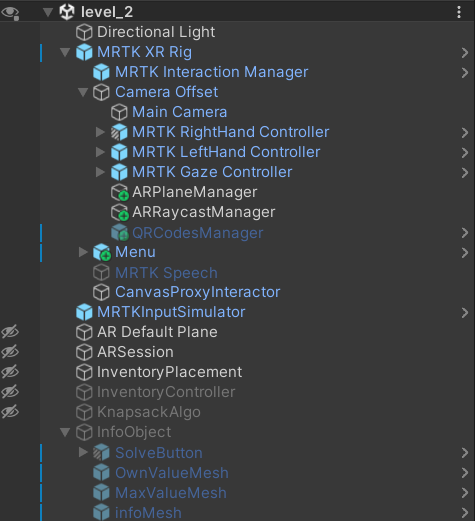
\includegraphics[scale=0.8]{images/Level2Hirarchy}
    \caption{Hierarchie des Knapsack-Problem Levels im Unity Editor.}
    \label{fig:level2_hierarchy}
\end{figure}

In dieser Abbildung ist der Aufbau und Inhalt der 2. Szene\footnote{Unity \cite{Scene}} also dem Knapsack-Problem Level
zu sehen. Wie zu sehen ist besteht die Szene für dieses Level aus mehreren wichtigen Unity Game Objekten. Darunter
sind die folgenden:

\begin{itemize}
    \item \textbf{level-2:} Die Scene in der Alle Unity-Game-Objekte enthalten sind.
    \item \textbf{MRTK XR Rig:} Das Objekt in dem die Hauptkomponenten wie z.B.: \textit{Main Camera, MRTK Interaction
    Manager, Alle Manager, etc... } für die AR-Applikation enthalten sind.
    \item \textbf{AR Default Plane:} In der Augmented Reality (AR)-Entwicklung bezieht sich ein Plane\footnote{Unity \cite{Plane}} normalerweise
    auf eine erkannte horizontale Fläche in der realen Welt, auf der virtuelle Objekte platziert werden können. Diese
    Flächen können zum Beispiel Tische, Böden oder andere ebene Oberflächen sein. Das Erkennen und Tracking von Planes
    ist entscheidend, um AR-Objekte realistisch in die Umgebung zu integrieren.
    \item \textbf{ARSession:} In Unity und AR Foundation bezieht sich die "ARSession" im Allgemeinen auf die
    Hauptkomponente, die die AR-Funktionalitäten steuert und koordiniert.
    \item \textbf{InventoryPlacement:} Ist ein Game Objekt, dem das \textit{Knapsackscript.cs} Script zugewiesen ist und
    bei Szenen-Start aktiv ist. Dieses Game Objekt kümmert sich darum, dass zu Beginn der Szene für drei Sekunden lang
    nach Planes gescanned wird. Nach Abschluss dieser 3 Sekunden wird anschließend dann das Inventar auf dem Plane auf
    das der User schaut platziert.
    \item \textbf{InventoryController:} Das Game Objekt, dem das \textit{InventoryController.cs} Script zugewiesen ist
    und nach Abschluss des InventoryPlacement Scripts aktiviert wird. Dieses Game Objekt wird jeden Frame ausgelöst
    und überprüft ob ein mit QR-Code versehenes Item in dem 3D Inventar platziert wurde.
    \item \textbf{KnapsackAlgo:} Ist das Game Objekt, dem das \textit{KnapsackAlgo.cs} Script zugewiesen ist und bei
    drücken des \textit{SolveButtons} aktiviert. Bei aktivierung dieses Scripts wird der Knapsack Algorithmus
    ausgeführt und somit der maximale Wert, der Wert des selbst zusammengestellten Inventars und die Perfekte Lösung
    errechnet.
    \item \textbf{InfoObject:} Dieses Game Objekt ist eine Sammlung aus mehreren Unity Game Objekten. Dieses Objekt wird
    bei Ausführung des InventoryPlacement Scripts neben dem Inventar platziert. Es beinhaltet einen Button, der bei Knopfdruck
    das \textit{KnapsackAlgo} Game Objekt aktiviert, und 3 verschiedene TextMeshPros\footnote{Unity \cite{TextMesh}} die
    für die Ausgabe von Infos zuständig sind.
    Außerdem ist bei diesem GameObjekt gut die Strukturierung von Game Objekten in Unity zu sehen. Die drei TextMeshPros
    und der Button sind dem \textit{InfoObject} untergeordnet was bedeutet, dass diese vier Game Objekte \textit{Children}
    von dem \textit{InfoObject} sind. Das übergeordnete Game Objekt wird hier dann als \textit{Parent} bezeichnet.
\end{itemize}

In der Abbildung ist zu sehen, dass ein Paar Game Objekte ausgegraut und nicht ausgegraut sind und, dass neben ein paar Game Objekten ein durchgestrichenes Auge zu sehen ist.
Wenn ein Game Objekt im Unity Editor ausgegraut ist bedeutet das, dass dieses GameObjekt und somit alle angehängiten Scripts von diesem Game Objekt deaktiviert sind.
Das bedeutet, dass dieses Game Objekt samt allen Scripts zu Szenenbeginn nicht aufgerufen und somit auch nicht ausgeführt werden. Nicht ausgegraute Game Objekte widerum sind
daher genau das Gegenteil. Das beudetet, dass das Game Objekt selbst samt allen angehängiten Scripts alle aktiviert sind und somit zu Szenenbeginn aufgerufen und ausgeführt werden.

Wenn neben einem Game Objekt das durchgestrichene Auge zu sehen ist bedeutet das nur, dass dieses Game Objekt im Unity Editor nicht zu sehen ist. Andererseits, wenn kein Zeichen
neben dem Game Objekt zu sehen ist, ist dieses Objekt im Unity Editor sichtbar. Dies dient dazu, dass falls in der Unity Szene viele Game Objekte vorhanden sind, dass man
diejenige ausblendet die nicht im Editor sichtbar sein müssen wie zum Beispiel Tesh Meshes oder Lables.

\subsection{Verwendung von QR-Codes}
Im vorangegangenen Abschnitt wurde bereits darauf hingewiesen, dass QR-Codes in diesem Level verwendet werden,
um die verschiedenen Items zu repräsentieren. Diese QR-Codes spielen eine entscheidende Rolle, indem sie dazu dienen,
vielfältige Informationen zu den einzelnen Objekten zu speichern und sie anschließend in einer virtuellen Umgebung
abzubilden. Im folgenden Abschnitt möchten wir näher darauf eingehen, wie genau diese QR-Codes generiert werden
und welchen Zweck sie innerhalb der Augmented Reality (AR)-Applikation erfüllen. Hierbei wird insbesondere betrachtet,
wie die Generierung der Codes erfolgt und auf welche Weise sie innerhalb der Anwendung zur Interaktion mit den realen Objekten verwendet werden.

\subsubsection{Inhalt der QR-Codes}
Die Informationen, die in einem QR-Code gespeichert werden, sind begrenzt. In unserem Anwendungsfall wird lediglich eine
einzelne Zahl im Bereich von 1 bis 11 abgespeichert. Diese Zahlen repräsentieren die 11 verschiedenen Modelle, die wir
unterscheiden möchten. Da nur eine Zahl gespeichert wird, genügt ein QR-Code der Größe 21x21 Module (Version 1). Die
geringe Anzahl von Modulen ermöglicht eine schnellere Erkennung auch über größere Distanzen.
%TODO: Testen und Grafik erstellen um zu zeigen das es eine Rolle spielt welche version wir verwenden + wie groß die sind

Die zugehörigen Zahlen erhalten in der Software, genauer gesagt in der Klasse \textit{QRItem.cs}, einen Kontext. Der folgende Codeausschnitt zeigt dies:

\begin{lstlisting}[style=csharp, caption={}, label=code:update]
public class QRItem
{
    public struct QRData
    {
        public int id;
        public string name;
        public Vector3 position;
        public int weight;
        public int value;
    }

    public QRData qrData;

    public Dictionary<int, QRData> items = new Dictionary<int, QRData>()
    {
        {1, new QRData { id = 1, name = "Laptop", weight = 70, value = 100 }},
        {2, new QRData { id = 2, name = "Router", weight = 25, value = 50 }},
        {3, new QRData { id = 3, name = "Maus", weight = 20, value = 30 }},
        // ...
        {11, new QRData { id = 11, name = "Handy", weight = 30, value = 100 }}
    };

    public QRItem(int id)
    {
        items.TryGetValue(id, out qrData);
    }
}
\end{lstlisting}

In dieser Klasse wird ein Dictionary verwendet, das den Zahlen die folgenden Informationen zuordnet:

\begin{itemize}
    \item \textbf{Item Id:} Die numerische Kennung im QR-Code.
    \item \textbf{Item Name:} Die Bezeichnung des Items, das dieser QR-Code repräsentiert.
    \item \textbf{Item Position:} Die Position des Items in der virtuellen Umgebung.
    \item \textbf{Item Weight:} Das Gewicht des Items.
    \item \textbf{Item Value:} Der Wert des Items.
\end{itemize}

Diese Informationen spielen eine wesentliche Rolle in der weiteren Berechnung des Knapsack-Algorithmus.

\subsubsection{QR-Code Tracking}
Das Tracking der QR-Codes erfolgt mithilfe des \textit{QRCodeManager.cs} Skripts. Dieses Klasse ist ein Singleton, das
die Erkennung und Verfolgung der QR-Codes steuert.
Das folgende UML-Diagramm zeigt die wichtigsten Methoden und zusammenhängenden Klassen:
%TODO: Abbildung einfügen
Nach der Erkennung eines QR-Codes erfolgen eine Reihe von Schritten, um diese Informationen zu speichern, verarbeiten
und zuletzt darzustellen.
Hier eine kurze Übersicht:
%TODO: Übersicht einfügen

\subsection{Platzieren des Inventars}
In diesem Abschnitt wird die \textit{PlaceObjectOnLookedAtDesk} Klasse des \textit{AnchorScript.cs} beschrieben. Dieses Script
implementiert das Platzieren des 3D Objektes des Inventars auf einem Tisch und kümmert sich zusätzlich
um das aktivieren und deaktivieren sämtlicher Game Objekte um den weiteren Verlauf des Spiels.

\subsubsection{Startverzögerung}
\begin{lstlisting}[style=csharp, caption={}, label=code:Start]
void Start()
{
    StartCoroutine(DelayedStart());
}
\end{lstlisting}
Zu Begin des \textit{Knapsack-Problem-Levels} wird die \textit{Lebenszyklusmethode} \textbf{Start()} aufgerufen. Diese
Funktion startet dann den Coroutine \textbf{DelayedStart()}.\\

\begin{lstlisting}[style=csharp, caption={}, label=code:DelayedStart]
IEnumerator DelayedStart()
{
    yield return new WaitForSeconds(3.0f); // Adjust the delay time as needed.
    canStartScript = true;
}
\end{lstlisting}
Anschließend wird in dieser Funktion eine Verzögerung von 3 Sekunden durchgeführt und anschließend \textit{canStartScript}
auf true gesetzt. Dies ist deswegen wichtig, weil durch dieses Verzögerte starten, die \textit{Planes} in der Umgebung ohne
Zwischenwirkung gescannt werden können. Dadurch kann im folgenden Abschnitt die \textit{Lebenszyklusmethode} \textbf{Update()}
Funktion weiter ausgeführt werden kann.

\subsubsection{Frame-Aktualisierung um richtiges Plane zu finden}
\begin{lstlisting}[style=csharp, caption={}, label=code:Update]
void Update()
{
    if (!objectPlaced && canStartScript)
    {
        List<ARRaycastHit> hits = new List<ARRaycastHit>();
        // Use Camera.main.transform.forward as the ray direction
        if (raycastManager.Raycast(new Ray(Camera.main.transform.position, Camera.main.transform.forward), hits, TrackableType.Planes))
        {
            ARPlane closestPlane = FindClosestPlane(hits);
            if (closestPlane != null)
            {
                if (selectedDeskPlane == null || selectedDeskPlane != closestPlane)
                {
                    selectedDeskPlane = closestPlane;
                    lookStartTime = Time.time; // Start the timer when a new plane is selected.
                }
                float timeLookedAtPlane = Time.time - lookStartTime;
                if (timeLookedAtPlane >= requiredLookTime)
                {
                    PlaceObjectOnDesk(selectedDeskPlane);
                    objectPlaced = true;
                }
            }
            else
            {
                selectedDeskPlane = null;
            }
        }
        else
        {
            selectedDeskPlane = null;
        }
    }
}
\end{lstlisting}
\textbf{Erklärung:}
\begin{enumerate}
    \item \textbf{Bedingte Aktualisierung:} Die \textit{Update()} Funktion wird nur dann weiter ausgeführt, wenn das Inventar
    Objekt nicht bereits platziert wurde. Wenn das Inventar noch nicht platziert wurde und \textit{canStartScript = true}
    ergibt dann kann die Funktion weiter fortschreiten.
    \item \textbf{Raycasting auf Planes:} In jedem Durchlauf dieser Funktion wird immer ein Raycasting durchgeführt und
    anschließend alle Treffer dieser Raycasts in einem Array verspeichert.
    \item \textbf{Suche nach dem am kürzest entfernten AR-Plane:} Nachdem das Raycasting abgeschlossen ist, wird anschließend die
    \textbf{FindClosestPlane(hits)} Funktion mit allen zuvor gespeicherten hits aufgerufen.
    \item \textbf{Zeiterfassung für die Blickzeit:} Jeden Frame wird die Variable \textit{timeLookedAtPlane} um die aktuelle
    verstriche Zeit \textbf{float timeLookedAtPlane = Time.time - lookStartTime} aktuallisiert.
    \item \textbf{Platzieren des Objekts bei ausreichender Blickzeit:} Wenn die \textit{timeLookedAtPlane} die \textit{requiredLookTime}
    übersteigt wird anschließend die Funktion \textit{PlaceObjectOnDesk(selectedDeskPlane)} mit dem ausgewählten Plane
    ausgeführt um das Inventar zu platzieren. Zusätzlich wird die Variable \textit{objectPlaced = true} gesetzt um aus der \textit{Update()}
    Funktion zu kommen und die Überprüfungen somit zu stoppen.//
\end{enumerate}
Diese \textit{Lebenszyklusmethode} wird so lange ausgeführt, bis das Script beendet und somit das Inventar samt dem Info-Objekt
platziert wurde.

\subsubsection{Das am kürzesten entfernte Plane finden}
\begin{lstlisting}[style=csharp, caption={}, label=code:findclosestplane]
ARPlane FindClosestPlane(List<ARRaycastHit> hits)
{
    ARPlane closestPlane = null;
    float closestDistance = float.MaxValue;
    foreach (var hit in hits)
    {
        ARPlane plane = planeManager.GetPlane(hit.trackableId);
        if (plane != null)
        {
            float distanceToPlane = Vector3.Distance(Camera.main.transform.position, hit.pose.position);
            if (distanceToPlane < closestDistance)
            {
                closestPlane = plane;
                closestDistance = distanceToPlane;
            }
        }
    }
    return closestPlane;
}
\end{lstlisting}

\textbf{Erklärung:}
\begin{enumerate}
    \item \textbf{Variablen Initilaisierung: }Zu Beginn der Funktion wird das \textit{closestPlane} als \textit{null}
    deklariert und die momentan kürzeste Distanz zu einem Plane wird in der \textit{closestDistance} Variable gespeichert.
    \item \textbf{Suche nach dem kürzesten AR-Plane:} Anschließend wird mit Hilfe einer \textit{foreach-Schleife} die
    Liste alle hits durchlaufen. In dieser Schleife wird dann immer das aktuelle AR-Plane anhand der \textit{trackableId}
    herausgenommen um es im weiteren Funktionsablauf zu bearbeiten.
    \item \textbf{Berechnung der Distanz:} Anhand des herausgenommenem AR-Plane wird nur die Distanz von diesem Plane zu
    zu Kamera Position berechnet.
    \item \textbf{Vergleich der Distanzen:} Der letzte Schritt des Schleifendurchlaufs ist, dass die aktuelle berechnete
    Distanz mit der davor gespeicherten \textit{closestDistance} verglichen wird. Wenn die Distanz kürzer ist, als die
    zuvor gespeicherte AR-Plane wird die \texit{closestDistance} überschrieben und die neue kürzeste Distanz wird gespeichert//
\end{enumerate}

\subsubsection{Berechnung der Position und aktivierung/deaktivierung sämtlicher Objekte}
\begin{lstlisting}[style=csharp, caption={}, label=code:placeobject]
void PlaceObjectOnDesk(ARPlane deskPlane)
{
    qrCodesManager.SetActive(true);
    // Calculate the object's position above the center of the plane.
    Vector3 objectPosition = deskPlane.center + Vector3.up * heightOffset;
    // Calculate the rotation to rotate the object -90 degrees around the x-axis.
    Quaternion objectRotation = Quaternion.Euler(-90f, 0f, 0f);
    // Instantiate the object with rotation.
    GameObject instantiatedObject = Instantiate(inventoryObject, objectPosition, objectRotation);
    // Set the scale of the instantiated object.
    instantiatedObject.transform.localScale = new Vector3(20f, 20f, 20f);
    // Spawn infoGameObject (Two TextMeshes and button for Knapsack Algorithm)
    Vector3 infoObjectPosition = objectPosition - Vector3.forward * 4.415f + Vector3.right * 0.4f;
    infoObject.transform.position = infoObjectPosition;
    infoObject.SetActive(true);
    // Set the inventoryObject in the InventoryController
    inventoryController.SetInventoryObject(instantiatedObject);
    // Enable the InventoryController
    inventoryController.gameObject.SetActive(true);
    // Set the visibility of the planes.
    planeManager.planePrefab.SetActive(false);
    // Disable this script so it won't run again.
    gameObject.SetActive(false);
}
\end{lstlisting}

\textbf{Erklärung:}
\begin{enumerate}
    \item \textbf{Aktivierung von QR-Code Manager:} Zu Beginn dieser Funktion wird der QR-Code Manager aktiviert und
    somit auch das tracken von QR-Codes.
    \item \textbf{Berechnung der Objektposition und Rotation:} Anschließend wird von dem ausgewählten AR-Plane die
    Flächenmitte \textit{objectPosition} berechnet. Zusätzlich wird die Objekt Rotation von diesem Objekt auf der x-Achse
    festgelegt mittels \textit{Quaternion.Euler(-90f, 0f, 0f)}.
    \item \textbf{Instantiierung des Objekts:} Nach berechnung der Position und Rotation wird das Objekt jetzt durch
    die Verwendung der \textit{Instantiate} Funktion instanziiert und skaliert.
    \item \textbf{Platzierung des infoGameObjects:} Zusätzlich zu dem Inventar-Objekt wird das Position des \textit{Info-Objects},
    dass aus 2 TextMeshes und 2 Buttons besteht festgelegt und anschließend aktiviert, dass es für den Benutzer sichtbar ist.
    \item \textbf{Setzen des InventarObjekts im InventoryController:} Das platzierte Inventar-Objekte wird an den \textit{InventoryController}
    weitergeleitet und dort deklariert, dass auf das selbe Game Objekt zugegriffen wird und die Berechnungen davon stimmen.
    \item \textbf{Aktivierung des InventoryController:} Nachdem das Inventar und das InfoObject erfolgreich platziert wurden
    und das InventoryObject erfolgreich an den InventoryController übergeben wurde wird nun der InventoryController
    aktiviert.
    \item \textbf{Sichtbarkeit der Planes ausschalten:} Daher, dass alle AR-Planes mit einer Textur markiert wurden, diese
    aber nach erfolgreicher Platzierung der Objekte nichtmehr sichtbar sein müssen werden diese nun mit \textit{planeManager.planePrefab.SetActive(false)}
    deaktiviert und sind somit nichtmehr sichtbar.
    \item \textbf{Deaktivierung des Skripts:} Nach Abschluss all dieser Schritte wird nun das \textit{AnchorScript.cs}
    entgültig deaktiviert um weitere Ressourcenverbrauchende Aktuallisierungen zu stoppen.
\end{enumerate}

\subsection{Inventar-Controller}
In diesem Abschnitt wird genauer auf das InventarController Script eingegangen und erklärt wie dieses funktioniert.

%Hier Code einfügen hihi

\subsection{Knapsack-Algorithmus}
Im folgenden Abschnitt wird der Knapsack-Algorithmus allgemein erklärt, die Problemstellung verdeutlicht und die
Unterschiede der beiden möglichen Algorithmen erläutert. Außerdem wird darauf eingegangen, warum er so wichtig ist
und in welchen Anwendungen er zum Einsatz kommt. Zudem wird das \textit{KnapsackScript.cs} besprochen, welches
diesen Algorithmus implementiert, um den maximal erreichbaren Wert und die optimale Lösung zu finden.

Der Knapsack-Algorithmus ist ein häufig verwendetes Werkzeug in der Informatik, um das Problem der optimalen
Ressourcenallokation zu lösen. Dieses Problem tritt auf, wenn eine begrenzte Menge an Ressourcen so effizient wie
möglich genutzt werden soll, um einen bestimmten Nutzen oder Gewinn zu maximieren. Der Begriff "Knapsack" leitet sich
von der Idee ab, dass man versucht, einen Rucksack mit begrenztem Fassungsvermögen mit Gegenständen zu füllen, die
unterschiedliche Werte und Gewichte haben.

\subsubsection{Problemstellung}
Gegeben sei ein Rucksack mit begrenzter Kapazität und eine Menge von Gegenständen, von denen jeder einen bestimmten
Wert und ein bestimmtes Gewicht hat. Das Ziel besteht darin, die Gegenstände auszuwählen, die in den Rucksack passen
und den Gesamtwert maximieren.

\subsubsection{Algorithmus}
Der Knapsack-Algorithmus kann in verschiedenen Varianten implementiert werden, darunter der dynamische
Programmieransatz und der Greedy-Ansatz. Im dynamischen Programmieransatz wird eine Tabelle erstellt, um
Teilprobleme zu lösen und die optimale Lösung zu berechnen. Der Greedy-Ansatz hingegen wählt Gegenstände basierend
auf bestimmten Kriterien aus, um eine lokale Optimierung zu erreichen.

In unserem Kontext wurde der dynamische Programmieransatz implementiert, um den Knapsack-Algorithmus umzusetzen.
Der Code dafür ist in der Datei \textit{KnapsackScript.cs} zu finden, welche den maximal erreichbaren Wert und
die optimale Lösung berechnet.

\subsubsection{Anwendungen}
Der Knapsack-Algorithmus findet Anwendung in verschiedenen Bereichen, darunter Logistik, Finanzplanung,
Ressourcenmanagement und Netzwerkoptimierung. Beispielsweise kann er verwendet werden, um den effizientesten
Transport von Gütern mit begrenzten Kapazitäten zu planen oder in der Finanzplanung, um das Portfolio von
Investitionen zu optimieren.

\subsubsection{Funktionsaufruf}
\begin{lstlisting}[style=csharp, caption={}, label=code:init]
int maxValue = KnapsackMaxValue(out usedItems, out int coveredCapacity);
int inventoryValue = -1;
maxMesh.text = "Maximal erreichbarer Wert: " + maxValue.ToString();
\end{lstlisting}
\textbf{Erklärung:} Hier wird die Funktion aufgerufen und dem textMesh \textbf{maxMesh} wird dieser Wert zugewiesen um dem User diesen Wert darzustellen.\\

\subsubsection{Variablen Initialisierung}
\begin{lstlisting}[style=csharp, caption={}, label=code:variable]
int n = items.Count;
int[,] dp = new int[n + 1, capacity + 1];
bool[,] selected = new bool[n + 1, capacity + 1];
\end{lstlisting}
\textbf{Erklärung:} Die Initialisierung erstellt die notwendigen Arrays für die dynamische Programmierung.\\

\subsubsection{Dynamischer Knapsack Algorithmus}
\begin{lstlisting}[style=csharp, caption={}, label=code:dynamic]
for (int i = 0; i <= n; i++)
{
    for (int w = 0; w <= capacity; w++)
    {
        % Initialisierung der DP-Tabelle
        if (i == 0 || w == 0)
            dp[i, w] = 0;
        else if (items[i].weight <= w && i <= maxItems)
        {
            % Berechnung des neuen Werts, wenn das Item ausgewählt wird
            int newValue = items[i].value + dp[i - 1, w - items[i].weight];
            if (newValue > dp[i - 1, w])
            {
                dp[i, w] = newValue;
                selected[i, w] = true;
            }
            else
            {
                dp[i, w] = dp[i - 1, w];
                selected[i, w] = false;
            }
        }
        else
        {
            dp[i, w] = dp[i - 1, w];
            selected[i, w] = false;
        }
    }
}
\end{lstlisting}

\textbf{Erklärung:}
\begin{enumerate}
    \item \textbf{Iterationen durch die Items und Kapazität:} Die äußere Schleife durchläuft jedes Item
    (\texttt{i}) von 0 bis zur Gesamtanzahl der Items (\texttt{n}). Die innere Schleife durchläuft jede mögliche
    Kapazität (\texttt{w}) von 0 bis zur maximalen Kapazität des Rucksacks.

    \item \textbf{Initialisierung der DP-Tabelle:} Wenn \texttt{i} oder \texttt{w} 0 ist, wird der Wert in der
    DP-Tabelle auf 0 gesetzt. Dies liegt daran, dass es keine Items gibt oder die Kapazität des Rucksacks 0 ist.

    \item \textbf{Überprüfung, ob das Item ausgewählt werden kann:} Wenn das aktuelle Item ausgewählt werden
    kann (basierend auf Gewicht und maximaler Anzahl von Items), wird der neue Wert berechnet, wenn das Item
    ausgewählt wird.

    \item \textbf{Vergleich und Auswahl:} Der neue Wert wird mit dem Wert verglichen, wenn das Item nicht
    ausgewählt wird. Wenn der neue Wert größer ist, wird das Item ausgewählt (\texttt{selected[i, w] = true}),
    andernfalls wird das vorherige Ergebnis beibehalten (\texttt{selected[i, w] = false}).

    \item \textbf{Falls Item nicht ausgewählt wird:} Wenn das aktuelle Item nicht ausgewählt wird, wird der
    Wert in der DP-Tabelle auf den Wert gesetzt, den das Rucksack ohne das aktuelle Item in der vorherigen
    Iteration erreicht hat.\\
\end{enumerate}

\textbf{Bedeutung der DP-Tabelle:}
Die DP-Tabelle (dp) dient dazu, Teilprobleme zu lösen und die besten Ergebnisse für verschiedene Kombinationen
von Items und Kapazitäten zu speichern. Jeder Eintrag in der Tabelle repräsentiert den maximal erreichbaren Wert
für eine bestimmte Menge von ausgewählten Items und eine bestimmte Kapazität des Rucksacks.

Insgesamt ermöglicht dieser Algorithmus, die optimale Auswahl von Gegenständen zu finden, die in den Rucksack
passt, um den Gesamtwert zu maximieren.


\subsubsection{Backtracking, um ausgewählte Items und perfekt Lösung zu finden}
\begin{lstlisting}[style=csharp, caption={}, label=code:backtrack]
List<List<int>> tempUsedItems = new List<List<int>>();
int row = n;
int col = capacity;
while (row > 0 && col > 0)
{
    List<int> group = new List<int>();
    while (row > 0 && col > 0 && selected[row, col])
    {
        // Item zu ausgewählter Gruppe hinzufügen
        group.Add(items[row].id);
        col -= items[row].weight;
        row--;
    }

    // Hinzufügen der Gruppe zur Liste
    if (group.Count > 0)
    {
        tempUsedItems.Add(group);
    }

    // Fortfahren mit dem Backtracking
    if (row > 0 && col > 0)
    {
        row--;
    }
}
\end{lstlisting}

\textbf{Erklärung:}
\begin{enumerate}
    \item \textbf{Initialisierung von Zeilen- und Spaltenindizes:} Die Variablen \texttt{row} und \texttt{col} werden auf die letzte Zeile und Spalte der DP-Tabelle gesetzt.

    \item \textbf{Hauptschleife für Backtracking:} Die äußere Schleife wird durchlaufen, solange die Zeile und die Spalte größer als 0 sind.

    \item \textbf{Innere Schleife für Gruppenbildung:} Solange die Zeile und die Spalte größer als 0 sind und das Item in der DP-Tabelle ausgewählt wurde (\texttt{selected[row, col]}), wird das Item zur aktuellen Gruppe hinzugefügt, das Gewicht von der aktuellen Kapazität abgezogen, und die Zeile wird dekrementiert.

    \item \textbf{Hinzufügen der Gruppe zur Liste:} Wenn die Gruppe mindestens ein Item enthält, wird die Gruppe zur temporären Liste \texttt{tempUsedItems} hinzugefügt.

    \item \textbf{Fortfahren mit dem Backtracking:} Die Zeile wird dekrementiert, um das nächste ausgewählte Item zu finden.
\end{enumerate}

Diese Schritte werden wiederholt, bis alle ausgewählten Items gefunden sind und die temporäre Liste \texttt{tempUsedItems} alle ausgewählten Gruppen enthält.\\

\subsubsection{Gruppengröße berechnen}
\begin{lstlisting}[style=csharp, caption={}, label=code:maxgroup]
int maxGroupSize = 0;
foreach (var group in tempUsedItems)
{
    if (group.Count > maxGroupSize)
        maxGroupSize = group.Count;
}
\end{lstlisting}
\textbf{Erklärung:} Findet die maximale Gruppengröße.\\

\subsubsection{Temporäres Array umwandeln und das usedItems Array befüllen}
\begin{lstlisting}[style=csharp, caption={}, label=code:convert]
usedItems = new int[tempUsedItems.Count, maxGroupSize];
for (int i = 0; i < tempUsedItems.Count; i++)
{
    for (int j = 0; j < tempUsedItems[i].Count; j++)
    {
        usedItems[i, j] = tempUsedItems[i][j];
    }
}
\end{lstlisting}
\textbf{Erklärung:} Konvertiert die temporäre Liste von Gruppen in ein 2D-Array, um die ausgewählten Items also die perfekt Lösung zu speichern.\\

\subsubsection{Rückgabewert}
\begin{lstlisting}[style=csharp, caption={}, label=code:return]
return dp[n, capacity];
\end{lstlisting}
\textbf{Erklärung:} Gibt den Gesamtwert des besten Rucksacks zurück.\\

\subsection{Darstellung der perfekten Lösung}
Um die perfekt Lösung nach der Berechnung erfolgreich darzustellen wird in diesem Abschnitt auf die \texit{PLACEHOLDES} Funktion des
\textit{KnapsackScript.cs} eingegangen um die errechnete Lösung nach dem drücken des \textit{SolveButton} anzugeigen

\subsection{Berechnen des eigenen Inventars}
In diesem Abschnitt wird auf die Funktion \textit{KnapsackInventoryValue} des \texit{KnapsackScript.cs} eingegangen. Diese Funktion
berechnet das Inventar Value des selbst gebauten Inventars.

\subsubsection{Funktionsaufruf}
\begin{lstlisting}[style=csharp, caption={}, label=code:aufruf]
inventoryValue = KnapsackInventoryValue(inventory);
if (maxValue == inventoryValue)
{
    infoMesh.color = Color.green;
    infoMesh.text = "Maximale Punktzahl erreicht";
}
else
{
    infoMesh.text = "";
}
ownMesh.text = "Erreichter Wert: " + inventoryValue.ToString();
\end{lstlisting}
\textbf{Erklärung:}
\begin{enumerate}
    \item \textbf{Inventar Wert berechnen:} Die Funktion KnapsackInventoryValue wird mit dem übergebenem invetory aufgerufen und der Inventar Wert berechnet.
    \item \textbf{Ergebnis Handling:} Wenn der eigene Wert gleich dem Maximalen errechnetem Wert enspricht hat der Benutzer gewonnen. Anderenfalls wird dem \texit{infoMesh} der aktuelle Wert zugewiesen.
\end{enumerate}

\subsubsection{Code für die Berechnung des eigenen Inventars}
\begin{lstlisting}[style=csharp, caption={}, label=code:ownInventory]
int KnapsackInventoryValue(int[,] inventory)
{
    if(inventory == null)
    {
        throw new System.Exception("Inventory is null");
    }

    int totalValue = 0;

    foreach (var item in items.Values)
    {
        int itemId = item.id;
        int itemValue = item.value;

        for (int j = 0; j < inventory.GetLength(0); j++)
        {
            for (int k = 0; k < inventory.GetLength(1); k++)
            {
                if (inventory[j, k] == itemId)
                {
                    totalValue += itemValue;
                }
            }
        }
    }

    return totalValue;
}
\end{lstlisting}
\textbf{Erklärung:}
\begin{enumerate}
    \item \textbf{Überprüfung auf Null:} Die Funktion überprüft, ob das übergebene Inventar null ist. Falls ja, wird eine Ausnahme ausgelöst.

    \item \textbf{Initialisierung des Gesamtwerts:} Die Variable \texttt{totalValue} wird auf 0 initialisiert. Hier wird der Gesamtwert des Rucksackinventars gespeichert.

    \item \textbf{Durchlauf aller Gegenstände:} Die Funktion durchläuft alle Gegenstände im globalen \texttt{items}-Dictionary.

    \item \textbf{Extrahierung von Informationen:} Für jeden Gegenstand werden die ID (\texttt{itemId}) und der Wert (\texttt{itemValue}) extrahiert.

    \item \textbf{Durchlauf des Inventars:} Die doppelte Schleife durchläuft das gesamte Inventar (\texttt{inventory}) und prüft, ob der aktuelle Gegenstand vorhanden ist.

    \item \textbf{Berechnung des Gesamtwerts:} Wenn der Gegenstand im Inventar gefunden wird, wird sein Wert zum Gesamtwert (\texttt{totalValue}) addiert.

    \item \textbf{Rückgabe des Gesamtwerts:} Am Ende wird der Gesamtwert des Rucksackinventars zurückgegeben.
\end{enumerate}

\subsection{Unit-Tests}
Durch Hilfe von Unit-Tests wird versichert, dass der implementierte Knappsack-Algorithmus
richtig und performant funktioniert.
%Genauere Erklärung + Custom Code der UnitTests

\section{Performance}
Performance-Messung
